\documentclass[14pt]{article} 

\usepackage[lmargin=0.3in, rmargin=0.3in, tmargin=0.3in, bmargin=0.3in]{geometry}
\usepackage[english]{babel} 
\usepackage{lipsum} 
\usepackage{verbatim}
\usepackage{amsmath}
\usepackage{tikz}
\usetikzlibrary{positioning,arrows.meta,calc}
\usepackage{graphicx}
\graphicspath{{figures/}}
\usepackage{natbib} 


% Sans-serif Schriften (Helvetica)
\renewcommand{\familydefault}{\sfdefault}
\usepackage{helvet}
\usepackage{cmbright}

\newcommand\wordcount{
  \immediate\write18{texcount -inc -tex  -sub=section draft.tex | cut -c -70 - > words.sum }
  \verbatiminput{words.sum} 
}



\usepackage{hyperref} 

\hypersetup{
	hidelinks,
	breaklinks=true,
	bookmarksopen=false,
	pdftitle={Title},
	pdfauthor={Author},
}



\title{Active Vision: How Eye Movements Shape What We See} 

\author{Francesco Mannella\textsuperscript{1}*, Andrea Mattera\textsuperscript{1}*, Luca Tummolini\textsuperscript{1}*\\
    \textsuperscript{1}\textit{Consiglio Nazionale delle Ricerche}\\
Istituto di scienze e tecnologie della Cognizione\\
Roma, Italia} % Author affiliation
% \affiliation{*\textbf{Corresponding author}: francesco.mannella@cnr.it} % Corresponding author




\begin{document}
%TC:ignore
 \wordcount
%TC:endignore
\maketitle

%TC:break abstract
\begin{abstract}

\normalsize
Our eyes are always moving, constantly shifting what we see on our retina.
Nevertheless we perceive a seamless visual world.

Two main hypotheses explain how we perceive a stable visual world despite constant eye movements: retinotopic updating and spatiotopic updating.
Retinotopic updating suggests that our brains continuously adjust our perception based on changes happening directly on the retina.
Spatiotopic updating also proposes that our brains build a stable, "world-centered" map of our surroundings, keeping our perception consistent regardless of where our eyes are looking.
However, recent evidence increasingly favors the retinotopic hypothesis over the spatiotopic one.
Starting from the retinotopic hypothesis, but without shifting receptive fields, we propose an ideomotor explanation wherein visual stability is predicated on learned, aligned action-perception interactions.
This framework integrates saccades and pre- and post-saccadic retinal states into an ideomotor schema, conceptualizing them as actions, conditions, and effects.
Retinal states select saccades and address the effects those saccades are expected to produce; upon achievement, these effects become the conditions for subsequent saccades.
Acquired ideomotor chains reflect the affordances inherent within experienced visual scenes.
Stable perception is hypothesised to rest on the congruence between saccades and visual outcomes, learned during experience as an alignment of motor commands and resultant sensory inputs that reflects the interactive possibilities within the visual environment.
Critically, feedback correction is not necessary for this process.
We hypothesize that this ideomotor schema is neurally instantiated through the alignment of brain regions governing eye movements with those processing visual information, forming an ideomotor internal space.
Within this neural space, an action, its prompting conditions, and its anticipated visual outcome converge into a unique neural assembly spanning the eye-movement and visual regions.
These neural assemblies represent specific prototypes of retino-saccadic contingency patterns.
Similar contingency patterns are clustered within the space, such that both the saccadic and visual neural components maintain a common topology.
To demonstrate the functional validity of this mechanism, we present a computational model of voluntary saccades operating within simplified simulated visual environments.
This model reproduces key features of voluntary oculomotor behavior and offers a functional reading of the influence of the fronto-parietal network, specifically the frontal eye fields (FEF) and the lateral intraparietal cortex (LIP), on the superior colliculus (SC) in humans and primates. It gives the functional counterpart of remapping, a learned relation between a view, a saccade and its expected effect, and not its neural signatures: no receptive field shifts, and stability across different starting views is yet to be tested.
\end{abstract}

\tableofcontents

\section{Introduction}
\paragraph{Visual perception is based on saccades.} 
Our brains do not passively record a continuous ``video'' of what we see.
Instead, we actively build our visual experience from snippets of information gathered through rapid eye movements.
Imagine you're looking at a painting in a museum: you don't just stare blankly at the center.
Instead, your eyes are constantly jumping from one detail to another – the artist's signature in the corner, a particular face in a crowd scene, a splash of color in the background.
Each of these jumps is a saccade.
Each time your eyes land on a new point, the light reflecting off that part of the painting stimulates your retina, sending a new burst of information to your brain.
You don't consciously perceive the gaps or the blurriness that occur during those saccades \citep{bridgemanFailureDetectDisplacement1975,burrSelectiveSuppressionMagnocellular1994,bindaVisionSaccadicEye2018}.
Why? Does your brain cleverly stitch together snapshots to create a complete, detailed picture? Does it generate missing visual information, simulating a ``video'' recording?  This is the explanation preferred by one prevalent and widely accepted theory, which posits that our brains actively compensate for the constant shifts in our gaze \citep{sommerWhatBrainStem2004,sunCorollaryDischargeOculomotor2016, cavanaughSaccadicCorollaryDischarge2016}.
This theory suggests that we don't just receive visual information; instead, our visual system uses predictions generated by an internal model based on our voluntary eye movements to correct and stabilize the incoming visual input.
Essentially, as our eyes move, our brain uses the information about these movements and adjusts what we perceive, allowing us to experience a stable and continuous visual world even though the raw retinal image is constantly changing.

% \paragraph{Scan-path theory.
Alternative views consider visual perception as a process which integrates the sequence of visual changes from saccades and the motor programs that produce that sequence.
The Scan-path Theory highlights that visual perception is an active process, involving purposeful eye movements that are guided by internal cognitive models and goals.

\paragraph{Spatiotopic vs retinotopic hypotheses}


\paragraph{Location-based remapping vs feature-based remapping}
\citep{herwigWhenCirclesBecome2015}
A model which interprets both location-based remapping and feature-based remapping

The standard retinotopic hypothesis assumes that a retinotopic spatial representation is updated in order to compensate for retinal displacement.
In this view, predictive remapping of receptive fields (Duhamel et al 1992) or attentional pointers (Cavanagh et al 2010) keeps track of the location of objects in retinotopic space.
 

Here we propose instead that a single location of the aligned space is at once a condition, an effect and an action.
When a retinal state activates its location, the activity of that location pre-activates, in a generative way, two retinal regions: the region of the current stimulus (the condition) and the region where the stimulus will fall after the saccade (the effect).
The same activity selects the saccade; executing it ends the decision and resets the mechanism, and the corollary discharge is hypothesised to be the signal that resets it.
Nothing shifts. What looks like remapping, a cell responding at its future field before the saccade and at its current field after it, is the pairing of two stable retinal regions in one location, learned from experienced saccades.
We claim that this is a possible alternative to the shifting of receptive fields, not the only one, and that it can be implemented at the neural level.


\paragraph{Stable perception test} Once topological alignment is acquired, a following reinforcement learning discrimination paradigm based on rewarding a specific area of the visualised object (es.
upper corner of a triangle).
The ability to foveate the target despite changes in the starting condition of foveal stimulation is considered an operational definition of stability in spatial perception (Cf Rao et al 2016).


 
\paragraph{Topological Alignment hypothesis.} This hypothesis explains how goals guide the selection of saccadic eye movements within an ideomotor framework.
Its core idea is that we learn an internal neural space made of aligned maps where each aligned subregion encodes: a prototypical retinal state during fixation, a prototypical retinal state representing the visual effect of a saccade, and the motor command for that saccade.
This internal space is learned through an open-ended process guided by the  offered by experienced visual environments.
During this learning, bottom-up salience guides the formation of connections between specific visual events, the subsequent saccadic movements, and the resulting retinal activities after the saccades.
The topological nature of this internal representation enables generalization and interpolation across various sensory and motor options.
As a result this topological neural system approximates a continuous map of all possible contingencies between oculomotor movements and retinal effects.



\paragraph{Description of the following sections.}


\section{Neural substrates of visual perception
}
\begin{itemize}
    \item Top-down / bottom-up overt attention
    \begin{itemize}
        \item SC-FEF circuit for the interaction of top-down and bottom-up attention.
        \begin{itemize}
            \item     V1 salience information to SC
            \item FEF direct pathway to SC
            \item SC indirect pathway to FEF

        \end{itemize}
        \begin{itemize}
        \item     Remapping of FEF receptive fields.
    \end{itemize}
    \end{itemize}
    \item LIP is involved in visual attention.
    \begin{itemize}
        \item Remapping of LIP receptive fields.
    \end{itemize}

\end{itemize}
 
\section{Topological Alignment}
\label{sec:ta}

Topological Alignment (TA) is the hypothesis that visual stability and the guidance of saccades rest on one learned structure: a set of maps, one for the retinal view before a saccade, one for the saccade, one for the retinal view after it, that share a common topology and are aligned location by location.
We state it at three levels: what it does, how it could be implemented in the brain, and how it is formalised in the model of the next section.

\subsection{Functional level: a location is a condition, an action and an effect}

A location of the aligned space is at once the condition of a saccade, the saccade, and its effect.
A retinal state activates a location; the activity of that location pre-activates the retinal region of the current stimulus (the condition) and the retinal region where the stimulus is expected to fall after the saccade (the effect), and selects the saccade.
Anticipation is therefore an address, not a computation: the expected effect is the content stored at the location that the current view selects, and no module computes where an item will land.
Executing the saccade ends the decision and resets the mechanism; the corollary discharge is hypothesised to be the reset signal.
Once the saccade is made, the effect becomes the condition of the next one, so that experience is organised in chains of conditions, actions and effects, the ideomotor chains of the abstract.

\begin{figure}
    \centering
    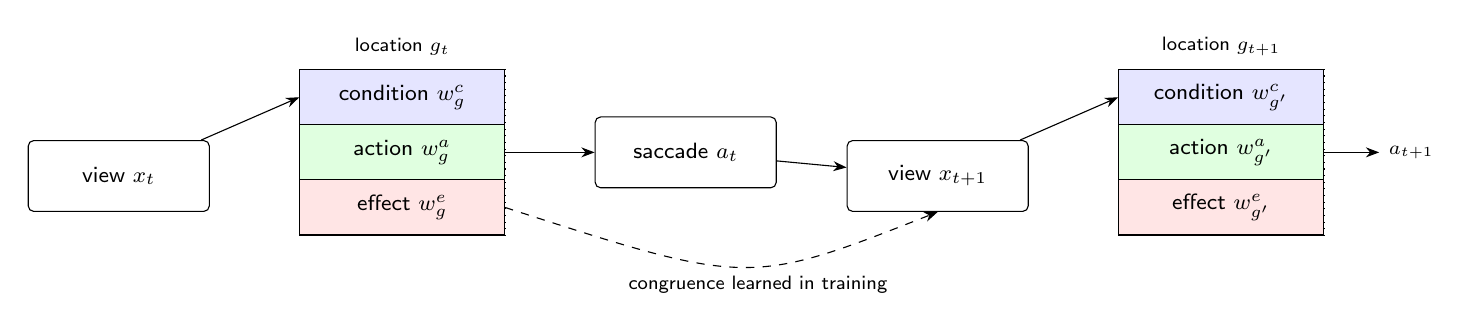
\begin{tikzpicture}[>=Stealth, font=\footnotesize,
      view/.style={draw, rounded corners=2pt, minimum width=2.3cm, minimum height=0.9cm, align=center},
      face/.style={draw, minimum width=2.6cm, minimum height=0.7cm, align=center},
      lab/.style={font=\scriptsize, align=center}]
      \node[view] (v0) at (0,0) {view $x_t$};
      \node[face, fill=blue!10] (c1) at (3.6,1.0) {condition $w^c_{g}$};
      \node[face, fill=green!12] (a1) at (3.6,0.3) {action $w^a_{g}$};
      \node[face, fill=red!10]   (e1) at (3.6,-0.4) {effect $w^e_{g}$};
      \node[lab, above=0.05cm of c1] {location $g_t$};
      \node[view] (sac) at (7.2,0.3) {saccade $a_t$};
      \node[view] (v1) at (10.4,0) {view $x_{t+1}$};
      \node[face, fill=blue!10] (c2) at (14.0,1.0) {condition $w^c_{g'}$};
      \node[face, fill=green!12] (a2) at (14.0,0.3) {action $w^a_{g'}$};
      \node[face, fill=red!10]   (e2) at (14.0,-0.4) {effect $w^e_{g'}$};
      \node[lab, above=0.05cm of c2] {location $g_{t+1}$};
      \draw[->] (v0) -- (c1.west);
      \draw[->] (a1.east) -- (sac);
      \draw[->] (sac) -- (v1);
      \draw[->] (v1) -- (c2.west);
      \draw[->] (a2.east) -- ++(0.7,0) node[right,lab] {$a_{t+1}$};
      \draw[dashed,->] (e1.east) .. controls (8,-1.4) .. (v1.south) node[pos=0.55,below,lab] {congruence learned in training};
      \draw[dotted] (c1.north west) rectangle (e1.south east);
      \draw[dotted] (c2.north west) rectangle (e2.south east);
    \end{tikzpicture}
    \caption{Ideomotor chain. A view activates a location whose three faces hold the condition, the saccade and the expected effect. The saccade is read from the action face; the expected effect (dashed) is the post-saccadic view that training has paired with that location. The view after the saccade activates the next location, so that the effect of one saccade is the condition of the next.}
    \label{fig:chain}
\end{figure}

Stability is the persistence of the neighbourhood relation between these three terms.
A view, the saccade selected by it and the view that follows keep addressing the same location, or locations that are close to each other, across experiences.
The relation is learned from the saccades that the agent itself makes.
Bottom-up salience drives exploration at first; the agent's competence, the degree to which the three maps agree at a location, then gates how much exploration is left and how plastic the location remains.
Goals (the locations selected by the conditions map) follow from the offered views and from the history of the episode, not from a position in external space.

\subsection{Neural level: aligned maps with a common topology}

We read the three maps as populations in the fronto-parietal network that governs saccades: the saccade map in the frontal eye fields (FEF) and, downstream, the superior colliculus (SC), the condition and effect maps in the lateral intraparietal cortex (LIP) and visual areas.
The alignment is the correspondence between neighbouring units of the three populations.
A neural assembly spanning them is a prototype of a retino-saccadic contingency, and neighbouring assemblies hold similar contingencies.
This reading is a hypothesis; the model does not simulate these areas, and the identification of the maps with FEF and LIP follows the functional correspondence only.

\begin{figure}
    \centering
    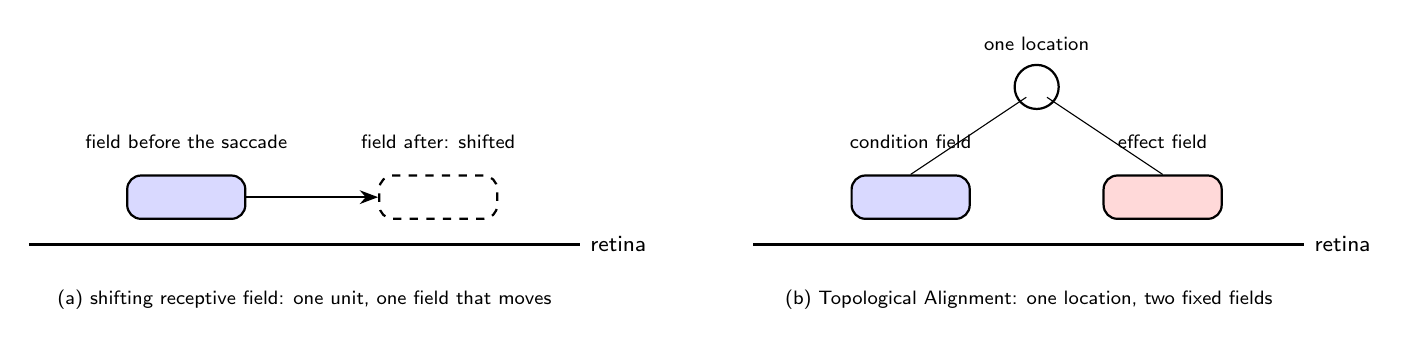
\begin{tikzpicture}[>=Stealth, font=\footnotesize,
      ax/.style={thick},
      rf/.style={draw, thick, minimum width=1.5cm, minimum height=0.55cm, rounded corners=5pt},
      lab/.style={font=\scriptsize, align=center}]
      \begin{scope}
        \draw[ax] (0,0) -- (7,0) node[right] {retina};
        \node[rf, fill=blue!15] (r0) at (2,0.6) {};
        \node[rf, dashed] (r1) at (5.2,0.6) {};
        \draw[->, thick] (r0.east) -- (r1.west);
        \node[lab] at (2,1.3) {field before the saccade};
        \node[lab] at (5.2,1.3) {field after: shifted};
        \node[lab] at (3.5,-0.7) {(a) shifting receptive field: one unit, one field that moves};
      \end{scope}
      \begin{scope}[xshift=9.2cm]
        \draw[ax] (0,0) -- (7,0) node[right] {retina};
        \node[rf, fill=blue!15] (q0) at (2,0.6) {};
        \node[rf, fill=red!15] (q1) at (5.2,0.6) {};
        \node[lab] at (2,1.3) {condition field};
        \node[lab] at (5.2,1.3) {effect field};
        \draw[thick] (3.6,2.0) circle (0.28) node (u) {};
        \node[lab] at (3.6,2.55) {one location};
        \draw[thin] (u.south west) -- (q0.north);
        \draw[thin] (u.south east) -- (q1.north);
        \node[lab] at (3.5,-0.7) {(b) Topological Alignment: one location, two fixed fields};
      \end{scope}
    \end{tikzpicture}
    \caption{Two readings of a cell that responds at its future field before a saccade and at its current field after it. (a) A receptive field moves toward the saccade target. (b) A single location is paired, through experienced saccades, with two stable retinal regions, the region of the stimulus that activates it and the region where that stimulus lands; nothing shifts.}
    \label{fig:remap}
\end{figure}

Two consequences follow for how such a system looks to an experimenter.
First, spatial order in a map does not show that a coordinate system is held and updated.
The maps are organised by the global content of the views and by their alignment with the saccade map, not by position, yet retinotopy appears in them as a by-product: position is one dimension of retina-centred input, and a saccade is a retinal vector, so a map aligned with the saccade map inherits order in retinal displacement.
We call this retinotopy indirect.
Second, what looks like remapping, a cell responding at its future field before the saccade and at its current field after it, can result from the pairing of two stable retinal regions at one location, without any receptive field shifting.
We claim this as a possible alternative to the shifting of receptive fields, not as the only one.
It predicts that (i) the layout of a map follows the statistics of the views it is trained on, (ii) the effect region of a location follows the landing place of the stimulus that activates the location, and this relation disappears if the pairing between conditions and effects is broken in training, and (iii) lesions of a neighbourhood displace a goal to neighbouring locations rather than to a wrong coordinate.
Section~\ref{sec:model} tests (ii); (i) and (iii) are not tested.

\subsection{Formal level: a lattice of aligned prototypes}
\label{sec:formal}

Let a lattice of $N$ locations carry three maps with prototypes $w^{c}_j$ (condition), $w^{a}_j$ (action) and $w^{e}_j$ (effect), $j=1,\dots,N$.
For a view $x$, the goal is the winner of the conditions map,
\begin{equation}
g(x)=\arg\min_j \lVert x-w^{c}_j\rVert^2 ,
\end{equation}
the saccade is the action prototype $w^{a}_{g}$ and the expected effect is $w^{e}_{g}$.
A location is stable for an experienced triple (view $x$, action $a$, post-saccadic view $y$) when the winners of the action and effects maps for $a$ and $y$ are close to $g(x)$ on the lattice,
\begin{equation}
\mu=\tfrac12\sum_{m\in\{a,e\}}\exp\!\left(-(d_m/\sigma_\mu)^2\right),
\end{equation}
with $d_m$ the lattice distance between $g(x)$ and the winner of map $m$.
The maps are trained so that this holds, with the supervised topological map loss
\begin{equation}
L=\tfrac12\sum_j \lVert x-w_j\rVert^2\,\phi_j\,\psi_j ,
\end{equation}
where $\phi_j$ is a Gaussian neighbourhood of the map's own winner, which gives each map its topology, and $\psi_j$ is a Gaussian of width $\sigma_t$ around the goal $g$, which is the anchor that aligns the three maps.
The anchor resembles an efference signal: it is written by the selected action and aligns the sensory maps to it.
It is an address on a shared lattice and carries no forward model of the image or of space.

\section{A computational model of visual attention based on Topological Alignment}
\label{sec:model}

\begin{figure}
    \centering
    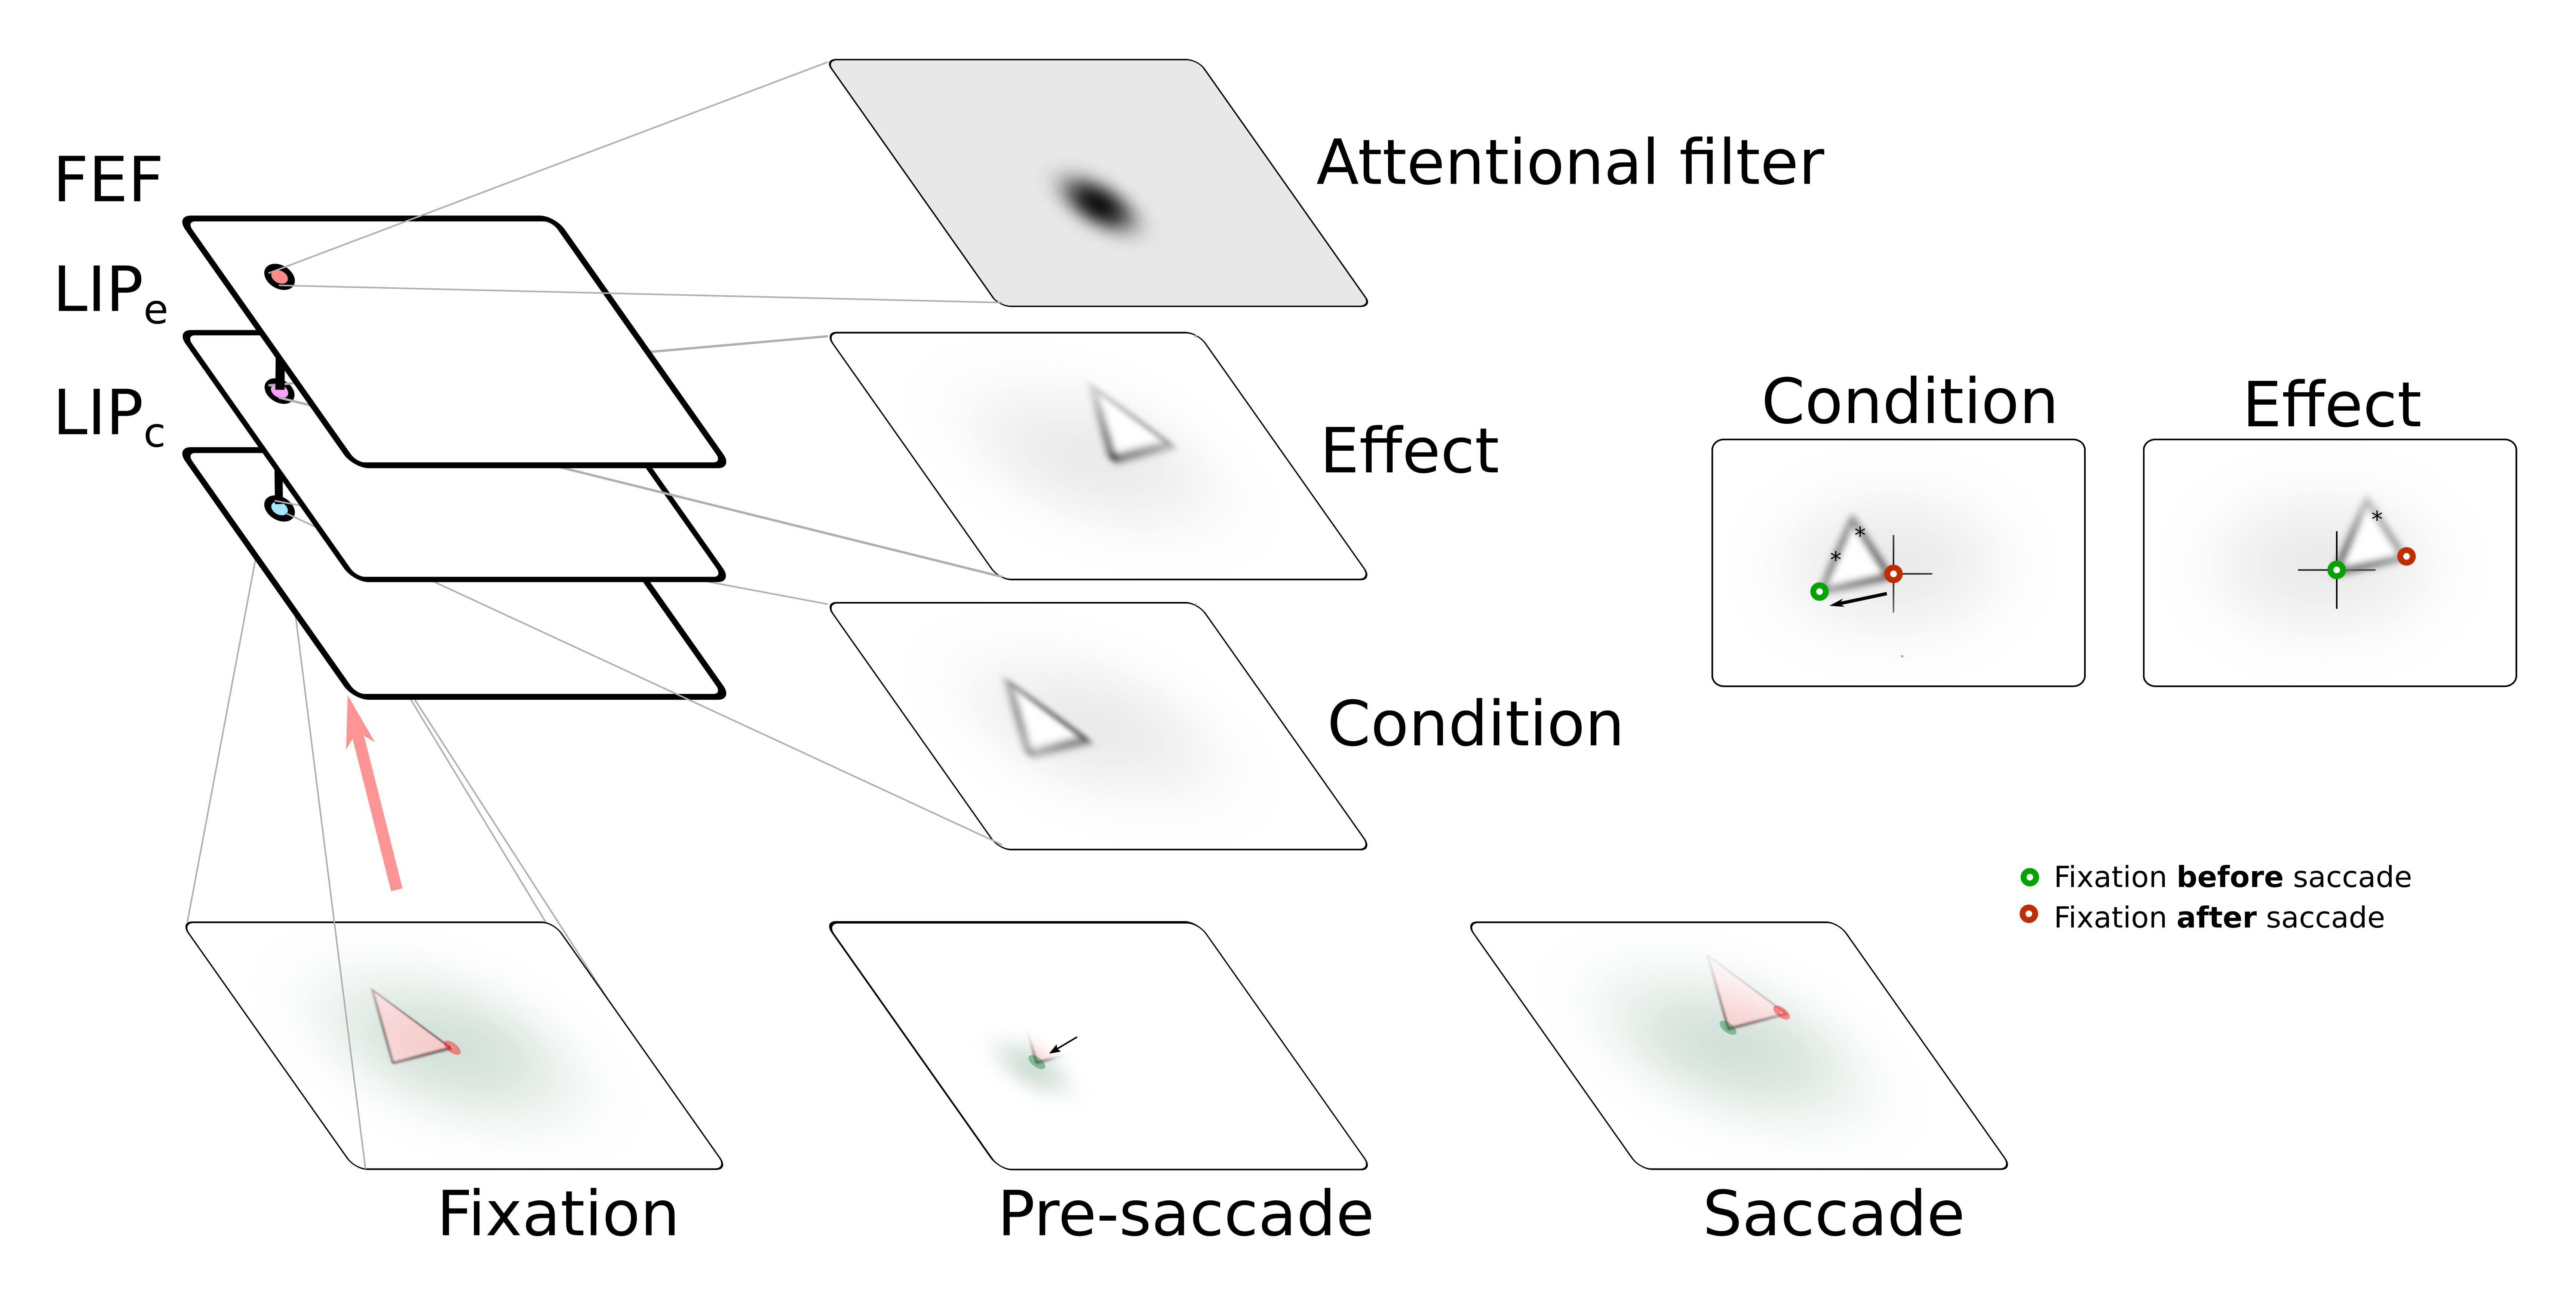
\includegraphics[width=0.8\textwidth]{meccanism}
    \caption{The mechanism. A column of units, one per lattice location, spans three layers: a condition layer that receives the retinal view at fixation (LIP$_\mathrm{c}$), an effect layer (LIP$_\mathrm{e}$) and an attentional layer that selects the saccade (FEF). Right: the condition is the view before the saccade, the effect is the view after it.}
    \label{fig:enter-label}
\end{figure}

\subsection{The model}

\subsubsection{Architecture}

An agent explores a simple coloured object, a triangle or a square, in a simulated $80\times80$ task space.
The agent sees an $80\times80$ retinal window centred on its gaze and a central fovea; the action is a displacement of the gaze.
A bottom-up saliency front end (Gabor filters on colour-opponent channels) turns the retinal image into a saliency map, which a Gaussian attentional mask centred on a retinal point multiplies; the next gaze position is the maximum of the result.
The offline controller holds three topological maps on a common $10\times10$ lattice: the visual conditions map (the foveal colour-saliency view before a saccade, $16\times16$ pixels), the attention map (the retina-normalised centre of the attentional mask that produced the saccade) and the visual effects map (the foveal view after it).
The winner of the conditions map for the current view is the goal; the saccade is the attention prototype at the goal.
Position in the external world is not available to the controller, and neither is eye position: the fovea is retina-centred and the action is a retinal vector.

\subsubsection{Learning}

Learning is offline, at the end of each epoch.
For each recorded saccade above a size threshold, the fovea two steps before is the condition, the fovea and attention centre two steps after are the effect and the action.
The three maps are updated with the loss of Section~\ref{sec:formal} (Adam), with the goal as the anchor.
A competence predictor, a logistic read-out of a Gaussian bump on the goal, is trained to output the match $\mu$ of each sample; its output is the local competence of a goal and its mean over locations is the global competence.
Competence modulates the neighbourhood width and the loss weight, so that plasticity shrinks as the maps agree.
The maps do not change during a saccade: no receptive field moves.

\subsubsection{Algorithm}

At the midpoint of each saccade the controller reads the fovea and finds the goal $g$ and its local competence $c$.
With probability $c$ it returns the attention prototype at $g$ as the new attentional centre; otherwise it returns a random centre on a ring around the retinal centre.
Exploration therefore fades as competence grows.
Three opt-in mechanisms, all part of the configuration used below, make the executed saccades faithful to the decisions and the scanpaths diverse:
\begin{itemize}
    \item goal inhibition multiplies the conditions distances by a Gaussian bump around each of the last three goals of the episode, which lengthens the scanpaths;
    \item hold fixation zeroes the gaze displacement on all steps except the decision step, so that each goal produces exactly one saccade and no salience-driven saccade undoes it;
    \item the orienting saccade adds one salience saccade with a uniform mask at the start of each episode, so that the first goal depends on the object's orientation.
\end{itemize}
At test time the learned model acts without exploration, always using the attention prototype at the winner, and the saliency inside the fovea is zeroed on decision steps so that a goal always moves the eye.

\begin{figure}
    \centering
    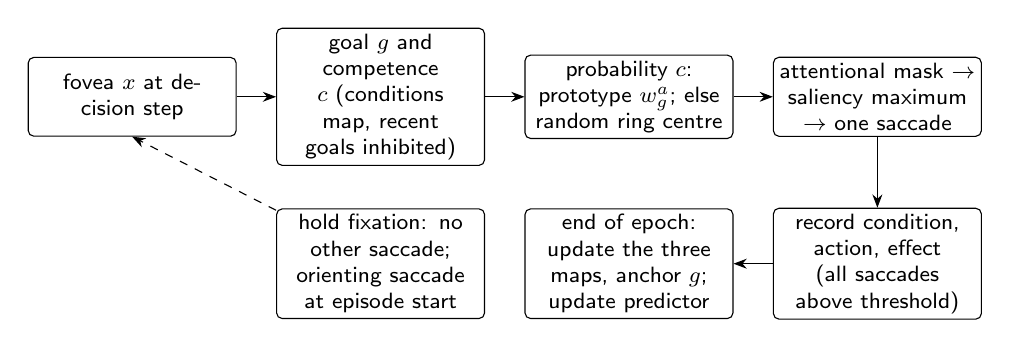
\begin{tikzpicture}[>=Stealth, font=\footnotesize,
      b/.style={draw, rounded corners=2pt, align=center, minimum height=1.0cm, text width=2.5cm, inner sep=2pt}]
      \node[b] (f) {fovea $x$ at decision step};
      \node[b, right=0.5cm of f] (g) {goal $g$ and competence $c$ (conditions map, recent goals inhibited)};
      \node[b, right=0.5cm of g] (p) {probability $c$: prototype $w^a_g$; else random ring centre};
      \node[b, right=0.5cm of p] (s) {attentional mask $\rightarrow$ saliency maximum $\rightarrow$ one saccade};
      \node[b, below=0.9cm of s] (r) {record condition, action, effect (all saccades above threshold)};
      \node[b, left=0.5cm of r] (u) {end of epoch: update the three maps, anchor $g$; update predictor};
      \node[b, left=0.5cm of u] (h) {hold fixation: no other saccade; orienting saccade at episode start};
      \draw[->] (f)--(g); \draw[->] (g)--(p); \draw[->] (p)--(s); \draw[->] (s)--(r); \draw[->] (r)--(u);
      \draw[->, dashed] (h) -- (f.south);
    \end{tikzpicture}
    \caption{One decision and the learning cycle of the model. Exploration fades with competence; hold fixation and the orienting saccade shape the executed saccades, not the learning rule.}
    \label{fig:loop}
\end{figure}

\subsection{Simulation setup}

Reference parameters: lattice of 100 locations, fovea $16\times16$ pixels, anchor width 4, neighbourhood baseline 0.5, $\sigma_\mu=10$, 1000 epochs of 20 episodes of 10 saccades.
The world alternates by epoch between the triangle and the square, so each update sees one object.
The configuration was selected on five seeds by the criteria that the goals of the two objects occupy separate regions of the conditions map, that scanpaths of different rotations share no goals, and that every goal saccade is executed.
We call it the champion; the choice is provisional.
Twenty champion runs (five from the selection and fifteen new seeds) were trained for the analysis of retinotopy.
For the remapping analysis the fovea sampled a wider retinal window, $48\times48$ or $64\times64$ pixels resized to the same $16\times16$ input, with three seeds each, because at $16\times16$ the saccade vectors of the attention prototypes (26 to 32 retinal pixels) leave the window.
Tests present each object at nine rotations (0 to 1.6 rad in steps of 0.2).
Scanpath measures: kNN purity (share of goals whose nearest goal in another test belongs to the same object), the share of test pairs with a common goal (rotations equivalent under the object's symmetry excluded), and the number of distinct goals per test.
Retinotopy is measured with a black-box spot probe, as an experimenter would map receptive fields: Gaussian spots at known positions, soft readout, a receptive-field centre per unit, and the rank correlation $\rho$ between lattice distance and receptive-field distance, with $z$ against permutations of the centres and a control with shuffled pixel layouts.
A phase-encoded probe (sweeping bars and an expanding ring) is a second, independent mapping.
Rules were fixed before the runs where stated; analyses without a prior rule are marked as post hoc.

\subsection{Behavior of the model}

\subsubsection{Aligned maps and scanpaths}

With the reference parameters (no inhibition or hold fixation, three seeds) the maps are well ordered in prototype space (Spearman correlation between lattice and prototype distance 0.89 on the conditions map, attention-map topographic error 0.07) and competence is about 0.73 to 0.78, with a seed spread as large as the differences among most hyperparameter settings (competence $0.727\pm0.063$ over five seeds).
The attention map is the weakest: 44 to 64\% of its units never win.
The first scanpaths locked onto 2 to 3 goals.
Goal inhibition lengthened them to 5 or 6, and exposed a failure of the control loop: after each decision the attention mask resets to a nearly flat distribution, so the next salience-driven saccade undid 33 to 43\% of the goal saccades, and the recorded effect was not the effect of the addressed saccade.
Hold fixation removed the reversals but made all scanpaths start from one shared goal (pairs sharing 0.68), and the orienting saccade removed the shared start (10 to 13 distinct first goals instead of 1 to 4).
In the champion configuration, objects are separated (purity 0.94), 5.4 distinct goals are visited per test, 20\% of test pairs share a goal (against 23\% in the earlier reference), every goal saccade is executed and no salience saccade follows it.
The earlier reference executed no saccade for 18\% of the goals and showed 25\% of salience saccades.

\begin{figure}
    \centering
    \includegraphics[width=\textwidth]{maps_champion.pdf}
    \caption{Learned maps of one run with the $48\times48$ window after 1000 epochs (seed 014142), on the $10\times10$ lattice. Left: prototypes of the conditions map, the view before the saccade, each tile the $48\times48$ window resized to $16\times16$. Centre: prototypes of the effects map, the view after the saccade, on the same grey scale. Right: the attention map, the retinal centre of the saccade at each location, linked by lattice adjacency. The dot of a location has the same colour in the three maps. The three maps share one lattice, so a location pairs a view, a saccade and the view after it. The run was chosen among the three runs of this window for the best worst case of three measures: ordering of the conditions map (Spearman correlation between lattice and prototype distance 0.76), ordering of the effects map (0.76) and agreement between the two layouts (0.66).}
    \label{fig:maps}
\end{figure}

\begin{figure}
    \centering
    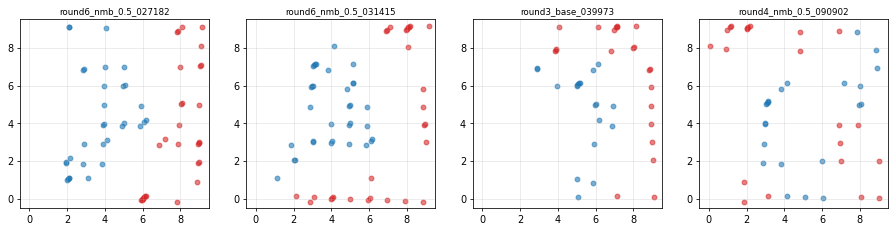
\includegraphics[width=\textwidth]{region_examples.png}
    \caption{Goals of all test scanpaths on the conditions lattice for four earlier reference runs (before hold fixation and orienting saccade); blue and red are the two objects. Goals of one object occupy a region separate from the other's.}
    \label{fig:regions}
\end{figure}

\begin{figure}
    \centering
    \includegraphics[width=\textwidth]{scanpath_champion.pdf}
    \caption{Executed fixations of one champion run (seed 031415) on each object at the nine test rotations, in task-space coordinates. Dots are the fixations at the 16 decision steps, coloured from first (dark, circled) to last (yellow); arrows are the saccades, each produced by one goal. At small rotations the fixations run along one edge of the object; from about 1 rad they move between the vertices or corners, and the path differs for each rotation. The run was chosen among the five champion runs with test scanpaths for legible paths (kNN purity 0.99, 5.2 goals per test); the run with the highest purity, seed 039973, produced paths of two or three fixations.}
    \label{fig:scanpath}
\end{figure}

\subsubsection{Indirect retinotopy of the maps}

The maps are trained on view content only, with no positional label, and the probe nevertheless finds retinotopy in all of them: $z>3$ in 40 of 40 maps of the 20 champion runs (median $\rho$ 0.82 for the conditions maps and 0.76 for the effects maps; median $z$ 45.9 and 40.2), and the phase-encoded probe agrees ($z>3$ in 40 of 40, median $\rho$ 0.54 and 0.58).
The order exceeds that of shuffled pixel layouts in 32 of 40 maps; in the other eight, all with low $\rho$, it is closer to prototype topography.
The run-to-run spread is large (conditions $\rho$ 0.55 to 0.87).
The probe cannot separate position from content in these views, so this result shows that spatial order is found, not how it arises.

\begin{figure}
    \centering
    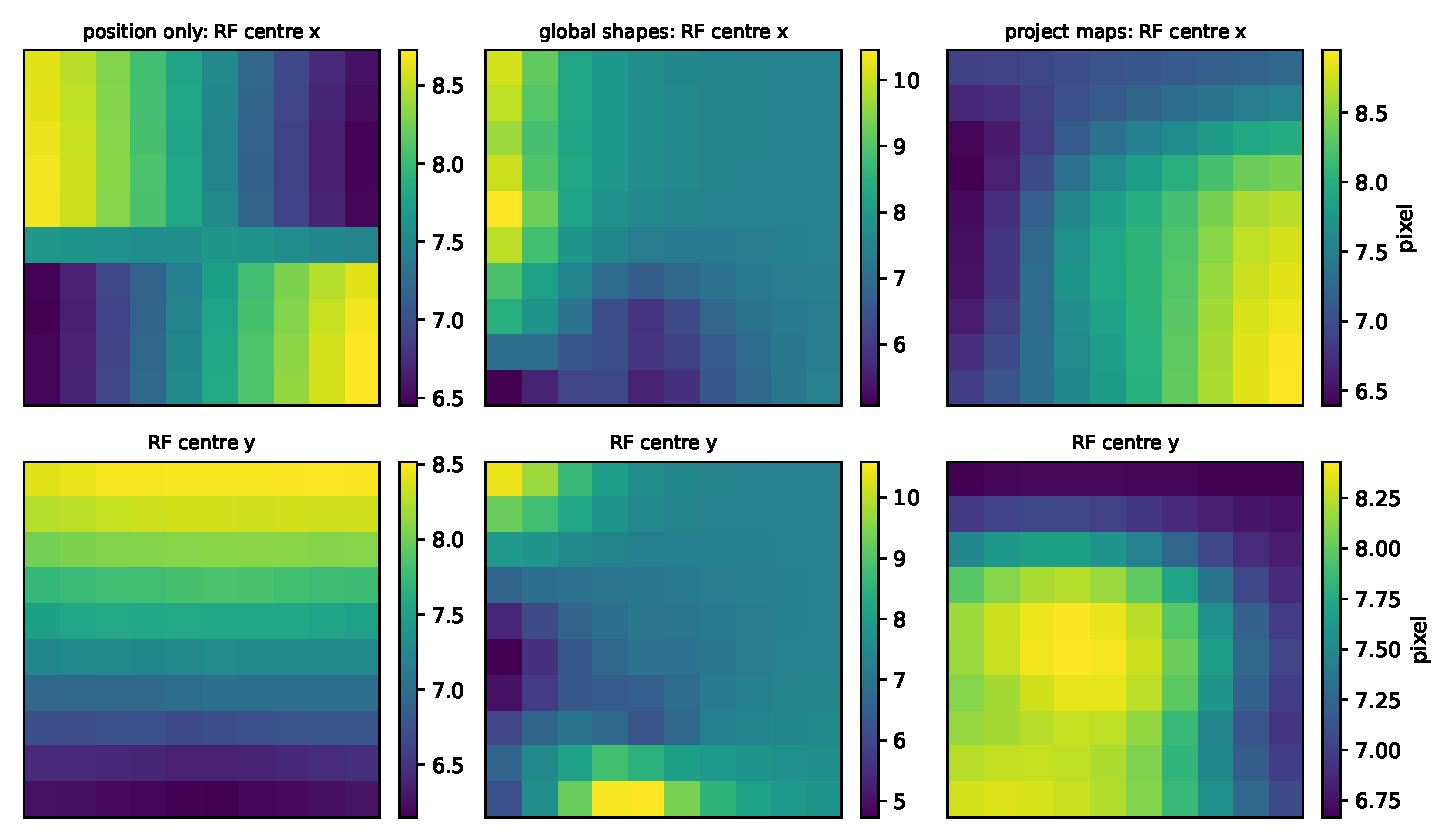
\includegraphics[width=\textwidth]{retinotopy_probe_maps.pdf}
    \caption{Receptive-field centres (horizontal, top; vertical, bottom) of the units of a $10\times10$ map found by the spot probe. Left: a map trained on positions only, retinotopic by design. Centre: a map trained on global shapes. Right: a map of the model, trained on view content only, with gradients over part of the lattice.}
    \label{fig:probe}
\end{figure}

\subsubsection{Remapping-like structure without shifting fields}

No field shifts in the model, since the maps are fixed during a saccade; the question is whether the pairing leaves a remapping-like signature at map level.
For each location, the post-saccadic field is the field of its effects unit and the saccade vector is the attention prototype.
With the $16\times16$ window the paradigm cannot be run (fraction of testable locations 0.00 to 0.02 against a minimum of 0.30), hence the wider windows (testable fraction 0.32 to 0.65 at 48 and 0.68 to 0.93 at 64, competence comparable to the narrow window).
Under the rule fixed beforehand, which compares the share of future-field responses among testable locations with the physiological range (0.27 to 0.82, Neupane et al. 2016) and with a control that permutes the effects units, the model does not reproduce predictive remapping: the shares (median 0.48 and 0.58) fall inside the range but are below the shuffled-pairing control in six of six runs, because the selection of testable locations aligns the response with the saccade whatever the pairing.
A statistic that tests the pairing directly, fixed after these results (post hoc), is the partial correlation between the effects field of the location activated by a spot and the place where the spot lands after the saccade, after removing the part of each that is linear in the spot's position, against a permutation of the effects units over locations.
At 48 pixels it is 0.46, 0.33 and 0.55 in three seeds ($p=0.003$, the smallest value possible with 300 permutations), and at 64 pixels 0.19, 0.06 and $-0.01$.
Retraining at 48 pixels with the effects states permuted across the batch, so that the condition and the effect of a location no longer come from the same view, gives 0.22, $-0.87$ and 0.03, and removes the full-size shift between the conditions and effects fields (regression ratio near 1 in two of the three unshuffled seeds, 0.24, 0.01 and 0.15 after shuffling).
At 48 pixels, therefore, the effects face of a location follows the landing of the stimulus that activates it, and this comes from the pairing in training, not from the lattice or from the read-out; at 64 pixels there is nothing to remove.
The effect is partial (the field centre stays 4 to 5 pixels from the landing place), and part of the forward relation between the fields is inherited from the conditions field alone.
A confirmatory test with five new seeds, paired and shuffled-pairing runs trained from the same seed, and its rules fixed before the runs, is in progress; the above is a pilot on three seeds per window.
The time course, latency and magnitude of remapping are not modelled.

\begin{figure}
    \centering
    \includegraphics[width=0.85\textwidth]{landing_pairing.pdf}
    \caption{Partial correlation between the effects field of the activated location and the landing place of the stimulus, per seed (lines join runs of the same seed). Blue: normal training. Orange: effects states permuted across the batch in training, which breaks the pairing. At 48 px the correlation is positive in all three seeds and disappears with shuffling; at 64 px it is near zero and shuffling does not remove it.}
    \label{fig:landing}
\end{figure}

\begin{figure}
    \centering
    \includegraphics[width=0.6\textwidth]{landing_example.pdf}
    \caption{Remapping-like structure in one run at window 48 (seed 022360). Top: three stimulus places (circles), selected as the places of the paired run whose landing is closest to the effects field of the location they activate (different locations, at least 4 px apart); the same places are shown for the run trained with shuffled effects. The saccade of the activated location takes each stimulus to its landing place (star), and the diamond is the effects field of that location. With paired training the diamonds lie within about 1 px of the stars; with shuffled effects the distances are 8.5, 5.5 and 1.2 px. The selection favours the paired run, so the typical case is in the bottom row: effects field centre against landing (x coordinate) over all testable places, with the line as equality. Over all testable places the mean distance between the effects field and the landing is 5.1 px for the paired run and 7.0 px for the shuffled run. No field moves in either run.}
    \label{fig:landing-example}
\end{figure}

\subsubsection{Stability}

The stable-perception test, foveating a rewarded part of the object from different starting views, has not been run.
A first measure, the invariance of the scanpath to the offset of the starting position of the retina, was 0.78 for the model against 0.91 for a control driven by salience alone, so the rule fixed beforehand failed and stability across starting views is not shown.
The model so far supports the learned relation between a view, a saccade and its effect, not stability as defined by the test.

\section{Discussion}

TA is not limited to the visual attention - oculomotor domain

TA is a general structure at least in fronto-parietal domains

TA is ideomotor anticipation of effects -- goals

TA in fromto-parietal loops produces neural representations which are grounded

\paragraph{Evidence and limits of the alternative to receptive-field shifting.}
In the trained maps, the retinal region of the effect of the location activated by a stimulus follows the place where the stimulus lands after the saccade, beyond what its pre-saccadic position alone predicts (partial correlation 0.33 to 0.55 in three runs with a 48 px retinal window); when the pairing between conditions and effects is broken during training, this relation disappears.
It is not found with a 64 px window, and it cannot be tested with a window of 16 px, where the landing falls outside the fovea.
The effect is partial.
This may reflect the capacity of the model, namely the number of units of the topology and the near-linear decoder from a location to a retinal prototype, which limit how sharply a location can pre-activate a retinal region; this has not been separated from the mechanism itself.
The time course, latency and response magnitude of remapping are abstracted away and are not addressed by the model.
The model shows that remapping signatures can arise without shifting receptive fields; it does not show that the nervous system works this way.

%------------------------------------------------

\section*{Acknowledgments} % The \section*{} command stops section numbering


So long and thanks for all the fish.

\section{Appendix}
\subsection{Model implementation}

\bibliographystyle{unsrtnat}
\bibliography{draft}

%----------------------------------------------------------------------------------------

\end{document}
